\chapter{システムコール呼び出し履歴を用いた検知手法の提案}

\section{新たな検知手法の必要性}
前章で述べたシンボルテーブルを用いてマルウェアの検知を行う検知手法では,stripコマンドを用いてシンボルテーブルを削除したり,検知条件となっている関数名を変更するといった攻撃者側による検知回避の対処が取られた際には有効な検知が行えないという課題がある.しかし,関数が呼び出すシステムコールの呼び出し順番は関数名の名称を変更しただけでは変化しない.straceと呼ばれる動作しているプロセスから呼び出されているシステムコールを追跡するコマンドを用いて,Miraiマルウェアのプログラムにおいて特徴的な動作を実装した内部関数に着目しこの関数から呼び出されるシステムコールの系列を用いた検知を行うことによって検知回避の対処がなされた場合でも検知が可能になる.


%書くべきこと
%スキャン動作に着目した理由

\section{Miraiの特徴的な動作に基づく検知条件知手法}
Miraiマルウェアは特徴的な動作として,サーバーにDDoS攻撃を行う動作の他にインターネットに公開されているホストに対して新たな侵入先を見つけるためにtelnetログインが可能な端末をスキャンする活動を行っている.また,MiraiはサーバにDDoS攻撃を行うプロセスとtelnetログインが可能な端末をスキャンする活動のプロセスは独立して動作しているため,プロセスは別々に存在している.DDoS攻撃を行うプロセスはDoS攻撃を行っている場合や,攻撃命令を待機している挙動など動的解析を行うタイミングによって,異なった解析結果が得られることが考えられる.しかし,スキャン活動を行うプロセスはログインできる端末を探索している挙動が主なため動的解析を任意のタイミングで行っても,共通している解析結果が得られると考えられる.DDoS攻撃を行うためのプロセスとスキャン活動を行っているプロセスについてstraceを用いてシステムコールを追跡したところ,DoS攻撃を行うプロセスは攻撃命令を待機している状態になるまでに呼び出されるシステムコールは様々なものがあった.しかし,スキャン活動を行っているプロセスはsendtoと呼ばれるソケットへメッセージを送るシステムコールを連続して呼び出していた.そのため,任意のタイミングでstraceをおこないシステムコールを追跡しても同様の結果を得ることができる.そのため,スキャン活動を行うプロセスに着目をしスキャン活動が呼び出すシステムコールの系列を用いた検知を行う.スキャン活動を行うプロセスのシステムコールの実行状況を追跡したところsendtoを連続して呼び出しており,sendtoによって送信されるメッセージの宛先アドレスが呼び出しごとに異なったアドレスであること,送信先のポートが23であったことからこのシステムコールを検知に用いる特徴とする.検知条件として3つの条件を定める.

\begin{enumerate}
\item sendtoのシステムコールが2回以上連続して呼び出されていること
\item sendtoによって送信先のポートが23であること
\item sendtoによって送信されるメッセージの宛先アドレスが呼び出しごとに異なったアドレスであること
\end{enumerate}


\section{誤検知の可能性}
前章で述べた検知条件をもとにマルウェア探索を行った際に,誤検知する場合として,以下の3つが考えられる

\begin{enumerate}
\item IoTデバイス上でsendtoの呼び出しが多いプログラムの実行
\item IoTデバイスから複数の端末に向けてメッセージを送信
\item IoTデバイスから複数の端末を遠隔操作しサーバー等の設定やログファイルを特定のサーバーへ転送
\end{enumerate}

straceを用いてシステムコールを確認し上記の動作が検知条件に一致するのか確認を行った.IoTデバイス上でsendtoの呼び出しが多いプログラムが実行されるプログラムとして,一定時間sendtoのみを呼び出すプログラムについて考える.sendtoが呼び出されるだけのプログラムでは,検知条件に一致しやすく誤検知する可能性がある.しかし,送信先のポートが23であり,送信されるメッセージの宛先がすべて別の宛先アドレスであるsendtoが呼び続ける正規プログラムが存在するとは考えにくい.IoTデバイスから複数の端末に向けてメッセージを送る動作として考えられるものが,wallやwriteなどIoTデバイスにtelnet,sshログインしている端末にメッセージを送るコマンドがある.wall,writeコマンドを実行してシステムコールを確認した結果が表2のようになる.%システムコールの結果を入れる
表2のようにsendtoを呼び出すことが確認されなかったため,IoTデバイスから複数の端末に向けてメッセージを送信する場合には誤検知することがない.IoTデバイスから複数の端末を遠隔操作する方法について,sshやtelnet,parallel-sshといったリモートシェルを用いて手動でコマンドを入力して端末を操作する場合とスクリプトファイルなどで端末を自動的に操作させる2種類がある.IoTデバイスから複数端末を手動でコマンドを入力してファイルの転送などを行いシステムコールを確認した結果,sendtoを連続では呼び出していなかった.スクリプトファイルを利用してファイルの転送を行う場合も,同様にsendtoを連続で呼び出していることを確認できなかった.sendtoだけを呼び出すプログラムをtelnet,sshを使用して端末上で実行した場合,本来はシステムコールであるsendtoが連続で呼び出されていたものがsendtoの次にwirteのシステムコールが呼び出されsendtoが2回以上連続で呼び出されていることが確認できなかった.sshやtelnetを利用して遠隔操作を行う場合や他の端末にメッセージを送信する場合にはsendtoが2回以上連続で呼び出されていることがないため誤検知することはないと考えられるため,これらの検知条件は妥当だと考える.

%実験環境も記載する
\section{straceコマンドによる監視対象のプロセスの実行速度の調査}

%あとで編集を行うようにする.
straceコマンドによってシステムコール呼び出し履歴を監視されるプロセスの実行速度が低下することが考えられる.そのため,straceコマンドによってプログラムの実行速度の変化を調べstraceによるシステムコールの監視動作がプロセスに与える実行速度の影響を調査した.使用するプログラムとしては,農林水産研究情報総合センターが定める,よく使用されるLinuxコマンド\cite{Linux}を使用した.cp,tar,df,ps,catの5つのコマンドを対象にstraceによるシステムコールの監視動作によるプロセスの実行速度の影響を調査した.実行したコマンドはは表\ref{tab:command}になる.
\begin{table}[h]
   \caption{実行したコマンド}
   \label{tab:command}
   \centering
    \begin{tabular}{clll}
     \hline
     \hline
     cat gpl-2.0.txt \\
     cp gpl-2.0.txt cp.txt \\
     ps -w \\
     df \\
     tar -zcvf gpl-2.0.tar.gz gpl-2.0.txt \\
     \hline
    \end{tabular}
\end{table}

  コマンドの引数にファイルが必要になる場合にはフリーソフトライセンスであるGPL2の内容が書かれているテキストファイルを使用した.表\ref{tab:command}%表を入れる
  の5つコマンドに対してのstraceコマンドを実行した場合の速度比較を行った.実行した結果が表\ref{tab:strace_result}になる.

\begin{table}[h]
   \caption{計測結果} 
   \label{tab:strace_result}
   \centering
  \begin{tabular}{|l|l|l|}
   \hline
   \multicolumn{1}{|c|}{} & 無為(秒)   & strace(秒) \\ \hline
   cat                    & 3.5730  & 3.6894    \\ \hline
   cp                     & 0.0048  & 0.2517    \\ \hline
   ps                     & 0.5134  & 10.9312   \\ \hline
   df                     & 0.6264  & 0.1212    \\ \hline
   tar                    & 0.57014 & 0.0294    \\ \hline
   \end{tabular}
\end{table}

システムコールの監視動作による速度はcatコマンドは3\%低下,cpコマンドは5079\%低下,psコマンドは2029\%低下,dfコマンドは417\%低下,tarコマンドは1839\%低下.この結果から,呼び出されるシステムコールによって速度の低下量は変化するがシステムコール監視動作によってプロセスの実行速度は低下することがわかった.システムコール監視対象となるプロセスが正常なプロセスだった場合,実行速度の低下がするため,マルウェア探索動作による1プロセスあたりのstraceの実行回数,アタッチする時間を短くする必要がある.


%行うことリスト
%\begin{enumerate}
%   \item よく実行されるコマンドのプロセスについて調べる
%   \item よく実行されるコマンドについてstraceをおこない実行する際のstraceのオーバーヘッドの量を調べる
%   \item コマンドに存在するシステムコールについてstraceを行い,straceのオーバーヘッドの量を調べる
%   \item 結果からstraceを使用することによってプロセスの実行時間が伸びるために提案システムでstraceを行う回数をへらすことを反す
%\end{enumerate}

%システムの概要図は挿入されているか
\section{システムコール呼び出し履歴を用いた検知手法の提案}
計算資源が潤沢でないIoTデバイス上でも実現可能な,Mirai亜種の動作を検知する軽量な動的解析に基づく検知システムを提案する.検知システムの概要を図\ref{fig:strace}に示す.Miraiはtelnetログインが可能な端末を探索するスキャン活動を行う機能を持ち,システムコールの一種であるsendtoを複数回連続で呼び出している.そこで動作しているプロセスからシステムコール呼び出し履歴を取得し,スキャン活動を行っているプロセスの動作を確認することでマルウェア感染の有無を判定する手法を以下に述べる.

\begin{enumerate}
 \item IoTデバイス上で動作を行うプロセスのホワイトリストを作成する.
 \item プロセスを監視し、作成されたホワイトリストをもとに記載がないプロセスを特定する.
 \item 特定した複数のプロセスに関して,straceを1秒間実行し検知条件に一致したシステムコール呼び出し呼び出し履歴があるか監視する.もし検知条件に一致したシステムコール呼び出し履歴があった場合にはマルウェアだと判断を行い通知を行う.
 
 \item 1プロセスあたりのstraceによるシステムコール監視動作の回数を減らすために,
 straceを実行したあとに監視動を中断する時間を設ける.マルウェアを検出するのに要する時間の最悪値を30秒とし,監視動作を中断する時間は以下の式で求める.
 \begin{eqnarray}
 中断時間  =  \frac{最悪値}{監視プロセス数}-1
 \end{eqnarray}
 \item 複数の監視対象となるプロセスに対してstraceを実行する.すべての監視対象となるプロセスに対してstraceを実行した場合には2に戻り繰り返す.
 \end{enumerate}
 
 検知システムとして前章で述べたシンボルテーブルを用いた検知システムに変更したものを利用した.

 %%%%%%%%%%%%%%%%%%%%%%%%%%%%%%%%%%%%%%%%%%%%%%%%%%%%%%%%%%%%%%%%%%%%%%
 % マルウェアの探索動作についてstraceをする回数を少なくしてもいい理由を書く
 % straceをするタイミングで検知できるかどうか変わらないのか変わらないならその理由を書く              
%%%%%%%%%%%%%%%%%%%%%%%%%%%%%%%%%%%%%%%%%%%%%%%%%%%%%%%%%%%%%%%%%%%%%%%

 \begin{figure}[h]
 \centering
    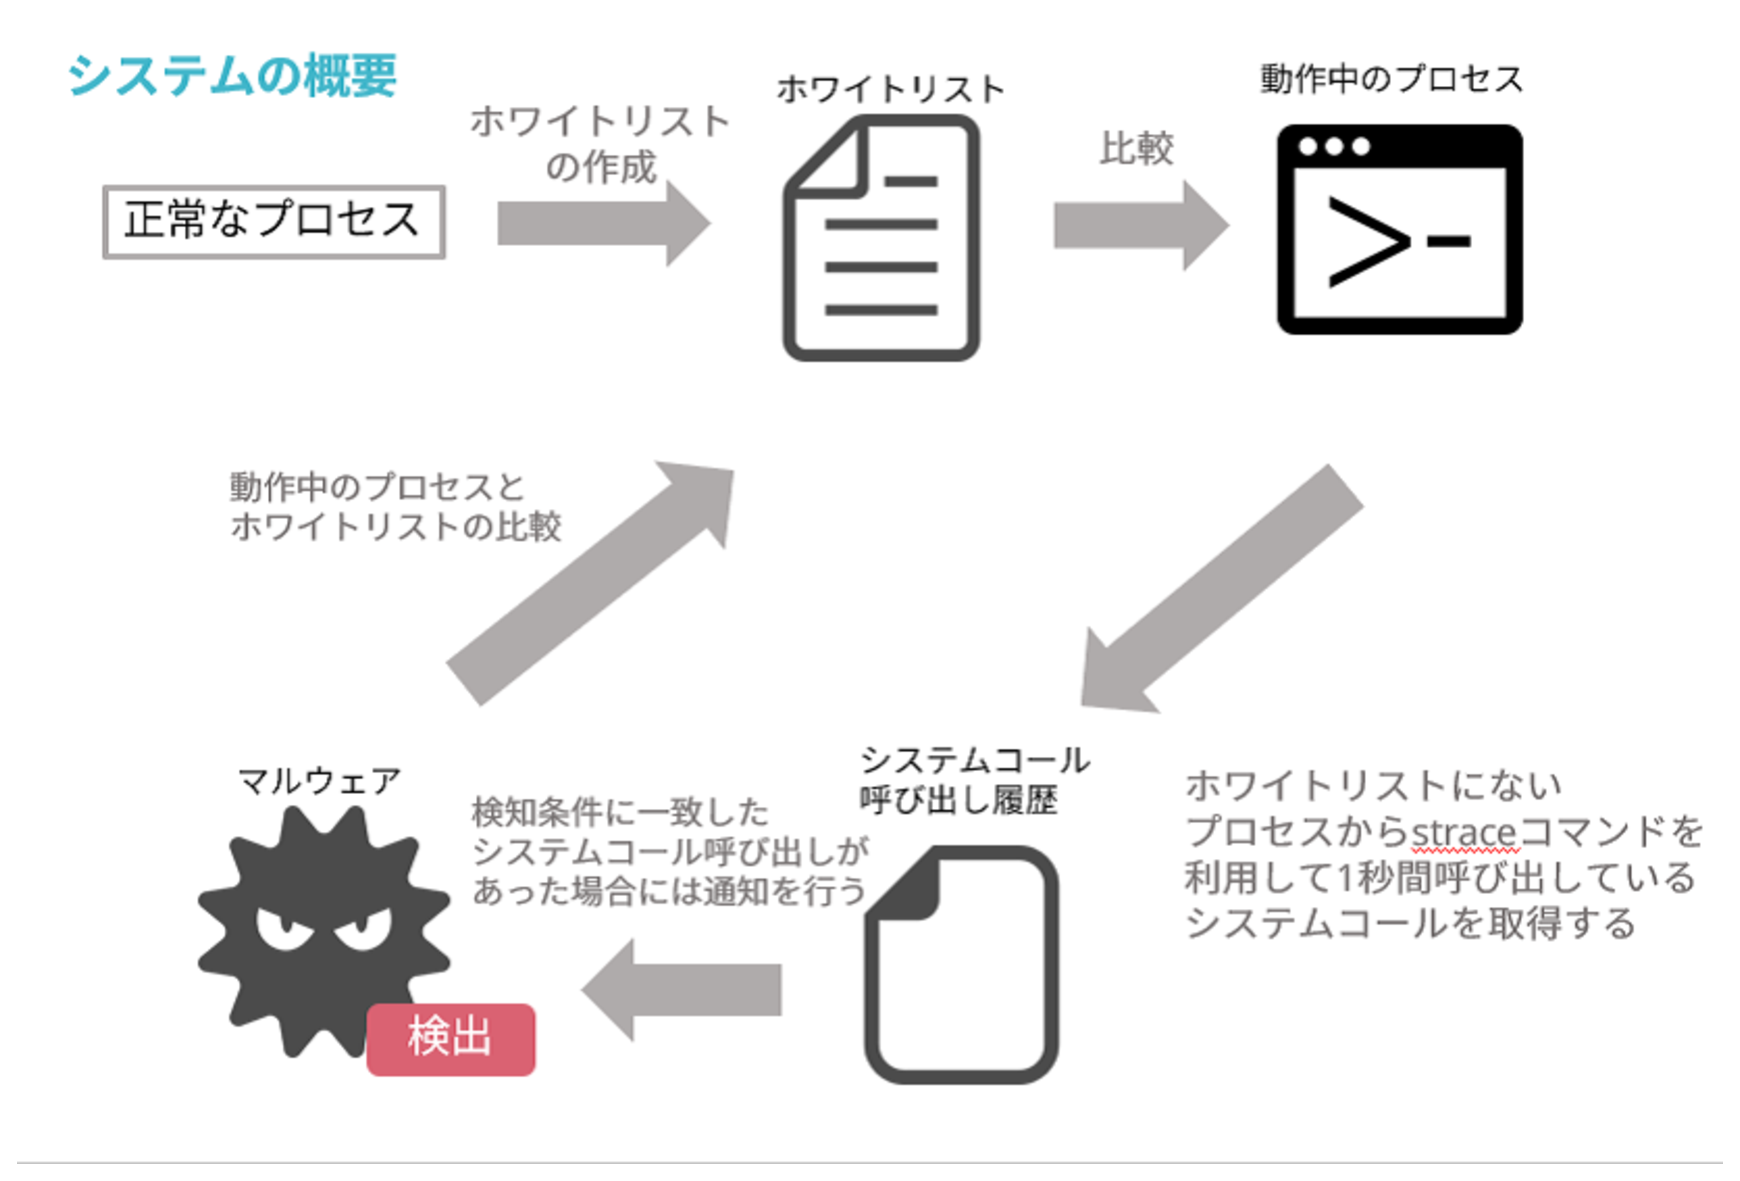
\includegraphics[width=100mm]{figures/strace.eps}
\caption{システムコール呼び出し履歴を用いた検知システムの概要}
\label{fig:strace}
 \end{figure}
 

